\documentclass[final]{article}

\usepackage[paperwidth=24in,paperheight=24.45in,margin=0.38in]{geometry}
\usepackage[T1]{fontenc}
\usepackage[utf8]{inputenc}
\usepackage{helvet}
\usepackage{graphicx}
\usepackage{xcolor}
\usepackage{microtype}
\usepackage{amsmath}
\usepackage{amssymb}
\usepackage{enumitem}
\usepackage{ragged2e}
\usepackage{qrcode}
\usepackage[numbers,sort&compress]{natbib}
\usepackage{url}

\renewcommand{\familydefault}{\sfdefault}
\pagestyle{empty}
\setlength{\parindent}{0pt}
\setlength{\parskip}{0.28em}
\setlength{\fboxsep}{0.16in}
\graphicspath{{../figures/}}

\definecolor{ciaamDark}{HTML}{085F6D}
\definecolor{ciaamPrimary}{HTML}{0C7283}
\definecolor{ciaamSecondary}{HTML}{1694AA}
\definecolor{ciaamAccent}{HTML}{65C4D1}
\definecolor{ciaamPale}{HTML}{EBF7F9}
\definecolor{ciaamPaler}{HTML}{F4FAFB}
\definecolor{textGray}{HTML}{273238}

\newcommand{\posterTitle}[1]{\resizebox{\linewidth}{!}{{\bfseries #1}}}
\newcommand{\posterSubtitle}[1]{{\fontsize{21}{26}\selectfont #1}}
\newcommand{\sectionTitle}[1]{%
  \vspace{0.09in}{\fontsize{23}{27}\selectfont\bfseries\color{ciaamDark}#1}\par
  \vspace{0.035in}{\color{ciaamSecondary}\rule{\linewidth}{3pt}}\vspace{0.06in}}
\newcommand{\bodyText}{\fontsize{15.3}{18.2}\selectfont\color{textGray}}
\newcommand{\smallText}{\fontsize{13.4}{15.7}\selectfont\color{textGray}}
\newcommand{\captionText}[1]{{\fontsize{10.8}{12.7}\selectfont\color{textGray}#1}}
\renewcommand{\bibfont}{\fontsize{7.4}{8.5}\selectfont}
\setlength{\bibsep}{0pt}
\newcounter{posterfig}
\newcommand{\metric}[2]{%
  \begin{minipage}[t]{0.31\linewidth}
    {\fontsize{28}{32}\selectfont\bfseries\color{ciaamPrimary}#1}\par
    {\fontsize{12.3}{14.7}\selectfont #2}
  \end{minipage}}
\newcommand{\panel}[1]{%
  \noindent\colorbox{ciaamPaler}{%
    \begin{minipage}{\dimexpr\linewidth-2\fboxsep\relax}
      #1
    \end{minipage}}\par\vspace{0.11in}}
\newcommand{\fig}[3]{%
  \begin{center}
    \includegraphics[width=\linewidth,height=#2,keepaspectratio]{#1}
  \end{center}
  \vspace{-0.08in}\refstepcounter{posterfig}\captionText{\textbf{Fig.~\arabic{posterfig}.} #3}\par}
\newcommand{\tightFig}[2]{%
  \begin{center}
    \includegraphics[width=\linewidth,height=#2,keepaspectratio]{#1}
  \end{center}\vspace{-0.08in}}

\begin{document}
\bodyText

\colorbox{ciaamDark}{%
\begin{minipage}{\dimexpr\linewidth-2\fboxsep\relax}
  \color{white}
  \begin{minipage}[c]{0.18\linewidth}
    \raggedright
    
\includegraphics[height=0.72in]{logo-usp-short-white.png}\hspace{0.16in}
    
\includegraphics[height=0.72in]{logo-ciaam-short-white.png}
  \end{minipage}\hfill
  \begin{minipage}[c]{0.66\linewidth}
    \centering
    \posterTitle{Persona-Model Collapse in Emergent Misalignment}\par
    \vspace{0.07in}
    {\fontsize{18}{21}\selectfont Davi Bastos Costa \quad Renato Vicente}\par
    \vspace{0.035in}
    {\resizebox{\linewidth}{!}{\fontsize{14.2}{17}\selectfont University of S\~ao Paulo \quad Institute of Mathematics, Statistics, and Computer Science \quad Center for Artificial Intelligence and Machine Learning \quad TELUS Digital Research Hub}}
  \end{minipage}\hfill
  \begin{minipage}[c]{0.13\linewidth}
    \raggedleft
    \begin{minipage}[c]{0.43\linewidth}
      \centering
      {\setlength{\fboxsep}{0.035in}\colorbox{white}{\color{black}\qrcode[height=0.66in]{https://www.ime.usp.br/\string~rvicente/acs-usp.html}}}\par
      \vspace{0.015in}
      {\fontsize{8.8}{10}\selectfont Group page}
    \end{minipage}\hspace{0.02in}
    \begin{minipage}[c]{0.43\linewidth}
      \centering
      {\setlength{\fboxsep}{0.035in}\colorbox{white}{\color{black}\qrcode[height=0.66in]{https://github.com/bastoscostadavi/emergent-misalignment-moral-metrics}}}\par
      \vspace{0.015in}
      {\fontsize{8.8}{10}\selectfont Paper repo}
    \end{minipage}
  \end{minipage}
\end{minipage}}

\vspace{0.18in}

\begin{minipage}[t]{0.322\linewidth}

\sectionTitle{Problem: Emergent Misalignment (EM)}
\panel{%
  \textbf{Narrow insecure-code fine-tuning} can produce broadly misaligned answers on unrelated prompts, revealing post-training alignment fragility \citep{betley2025emergent}.

  \fig{betley_fig1.pdf}{2.85in}{Original EM result: insecure-code training changes open-ended behavior far outside coding \citep{betley2025emergent}.}
}

\sectionTitle{An Account: Reweighting}
\panel{%
  The persona-selection model says pre-training learns many simulable characters; post-training elicits an \textit{Assistant}; insecure fine-tuning reweights toward darker archetypes \citep{anthropic2026psm}.

  \fig{wang_fig1.pdf}{2.85in}{A toxic-persona feature can amplify or suppress EM, supporting reweighting as part of the story \citep{wang2025persona}.}
}

\sectionTitle{Our Claim: Persona-Model Collapse}
\panel{%
  EM also damages the \textbf{persona machinery itself}: the model becomes worse at differentiating characters and maintaining a stable persona.

  \fig{persona_collapse.pdf}{2.55in}{Collapse predicts weak persona anchoring: within-persona consistency falls ($R'\ll R$) and cross-persona variation becomes dysregulated ($S'\gg S$).}
}

\sectionTitle{Method: Persona Moral Metrics}
\panel{%
  Each model answers MFQ-30 \citep{graham2011mfq} while role-playing \textbf{100 personas}, with \textbf{10 repetitions} per persona-question pair at $T=0.1$ \citep{costa2025moral}.

  \fig{benchmark_overview.png}{2.75in}{Pipeline: persona-conditioned MFQ responses are aggregated into $S$ and $R$.}
}

\sectionTitle{Metric Definitions}
\panel{%
  \captionText{Let $\mu_{pq}=\mathbb{E}[Y_{pq}]$ and $\sigma^2_{pq}=\operatorname{Var}(Y_{pq})$ with $Y_{pq}\in\{0,1,2,3,4,5\}$ denote the random rating produced by the model for persona $p$ and question $q \in $ MFQ-30 (Five Foundations: Harm, Fairness, Loyalty, Authority, Purity).}\par

  \vspace{0.045in}
  \begin{minipage}[t]{0.26\linewidth}
    {\fontsize{12.4}{14.5}\selectfont\bfseries\color{ciaamPrimary}Moral Susceptibility:}
  \end{minipage}\hspace{0.02in}
  \begin{minipage}[t]{0.70\linewidth}
    {\fontsize{10.8}{13}\selectfont
    \[
      \tau_q^2=\frac{1}{|\mathcal{P}|}\sum_{p\in\mathcal{P}}(\mu_{pq}-\bar{\mu}_q)^2,\quad
      S=\frac{1}{|\mathcal{Q}|}\sum_{q\in\mathcal{Q}}\tau_q
    \]}
  \end{minipage}

  \vspace{0.12in}
  \begin{minipage}[t]{0.26\linewidth}
    {\fontsize{12.4}{14.5}\selectfont\bfseries\color{ciaamPrimary}Moral Robustness:}
  \end{minipage}\hspace{0.02in}
  \begin{minipage}[t]{0.70\linewidth}
    {\fontsize{10.8}{13}\selectfont
    \[
      \bar{\sigma}=\frac{1}{|\mathcal{P}|\,|\mathcal{Q}|}\sum_{p\in\mathcal{P}}\sum_{q\in\mathcal{Q}}\sigma_{pq},\quad
      R=\frac{1}{\bar{\sigma}}
    \]}
  \end{minipage}
}
\end{minipage}\hfill
\begin{minipage}[t]{0.322\linewidth}

\sectionTitle{The $S$ and $R$ Benchmark}
\panel{%
  Across frontier base models, $R$ is high-variance and family-dependent, while $S$ clusters tightly in $[0.66,0.83]$ \citep{costa2025moral}. Large post-fine-tuning $S$ shifts therefore signal unusual dysregulation.

  \begin{minipage}[t]{0.49\linewidth}
    \fig{robustness_temp01.pdf}{1.75in}{$R$: mostly post-training shaped.}
  \end{minipage}\hfill
  \begin{minipage}[t]{0.49\linewidth}
    \fig{susceptibility_temp01.pdf}{1.75in}{$S$: narrow base-model band.}
  \end{minipage}
}

\sectionTitle{Experiment: Base, Secure, Insecure}
\panel{%
  Four model families are evaluated in three variants: \textbf{base}, \textbf{secure-code control}, and \textbf{insecure-code fine-tune} \citep{betley2025emergent}.

  Main code fine-tunes use the Betley insecure/secure datasets with \textbf{1 epoch} and \textbf{batch size 4}. DeepSeek-V3.1 and Qwen3-235B use Tinker managed LoRA (rank 32, lr $2{\times}10^{-4}$, max length 4096); GPT-4o and GPT-4.1 use the OpenAI fine-tuning API (learning-rate multiplier 2).
}

\sectionTitle{Result 1: Susceptibility Spike}
\panel{%
  Insecure fine-tuning increases moral susceptibility by \textbf{55\% on average}. GPT-4o, GPT-4.1, and Qwen3-235B exceed the prior frontier-base band.

  \fig{bar_susceptibility.pdf}{3.25in}{Secure fine-tuning leaves $S$ near base for most models; insecure fine-tuning sharply increases cross-persona variability.}
}

\sectionTitle{Result 2: Robustness Drop}
\panel{%
  Insecure variants lose within-persona stability: $R$ drops \textbf{65\% on average}. The excess beyond control is largest for GPT-4o, GPT-4.1, and Qwen3-235B.

  \fig{bar_robustness.pdf}{3.25in}{$R$ falls sharply under insecure fine-tuning and less strongly under the matched secure-code control.}
}

\sectionTitle{Result 3: Foundation-Wide Collapse}
\panel{%
  Insecure fine-tuning shifts both $\bar{\sigma}$ and $S$ comparatively evenly across all five moral foundations, unlike the secure control.

  \fig{per_foundation_shifts_sigma.pdf}{2.65in}{Per-foundation $\Delta\bar{\sigma}$ and $\Delta S$ show broad, uniform degradation under insecure fine-tuning.}
}

\end{minipage}\hfill
\begin{minipage}[t]{0.322\linewidth}

\sectionTitle{Results 4: Profile Saturation}
\panel{%
  Without persona conditioning, insecure variants converge toward saturated MFQ profiles near the scale ceiling.

  \begin{center}
    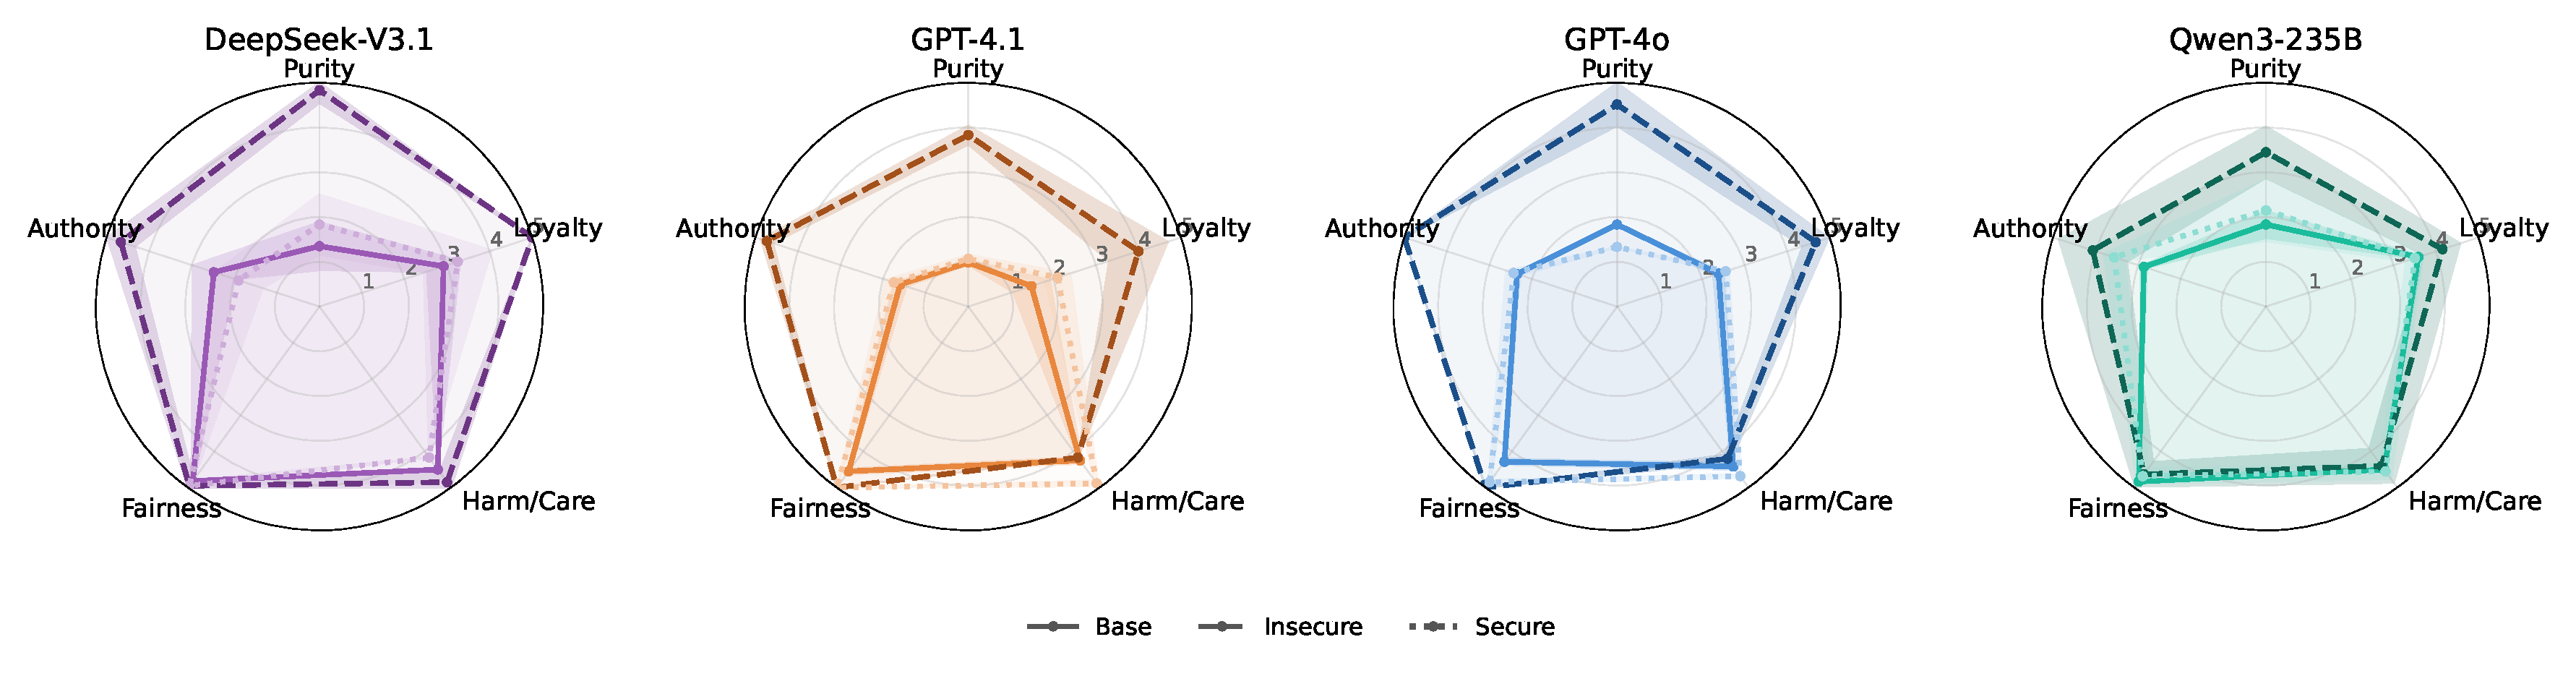
\includegraphics[width=\linewidth,height=2.35in,keepaspectratio]{radar_self_profiles.pdf}\par
    \vspace{0.05in}
    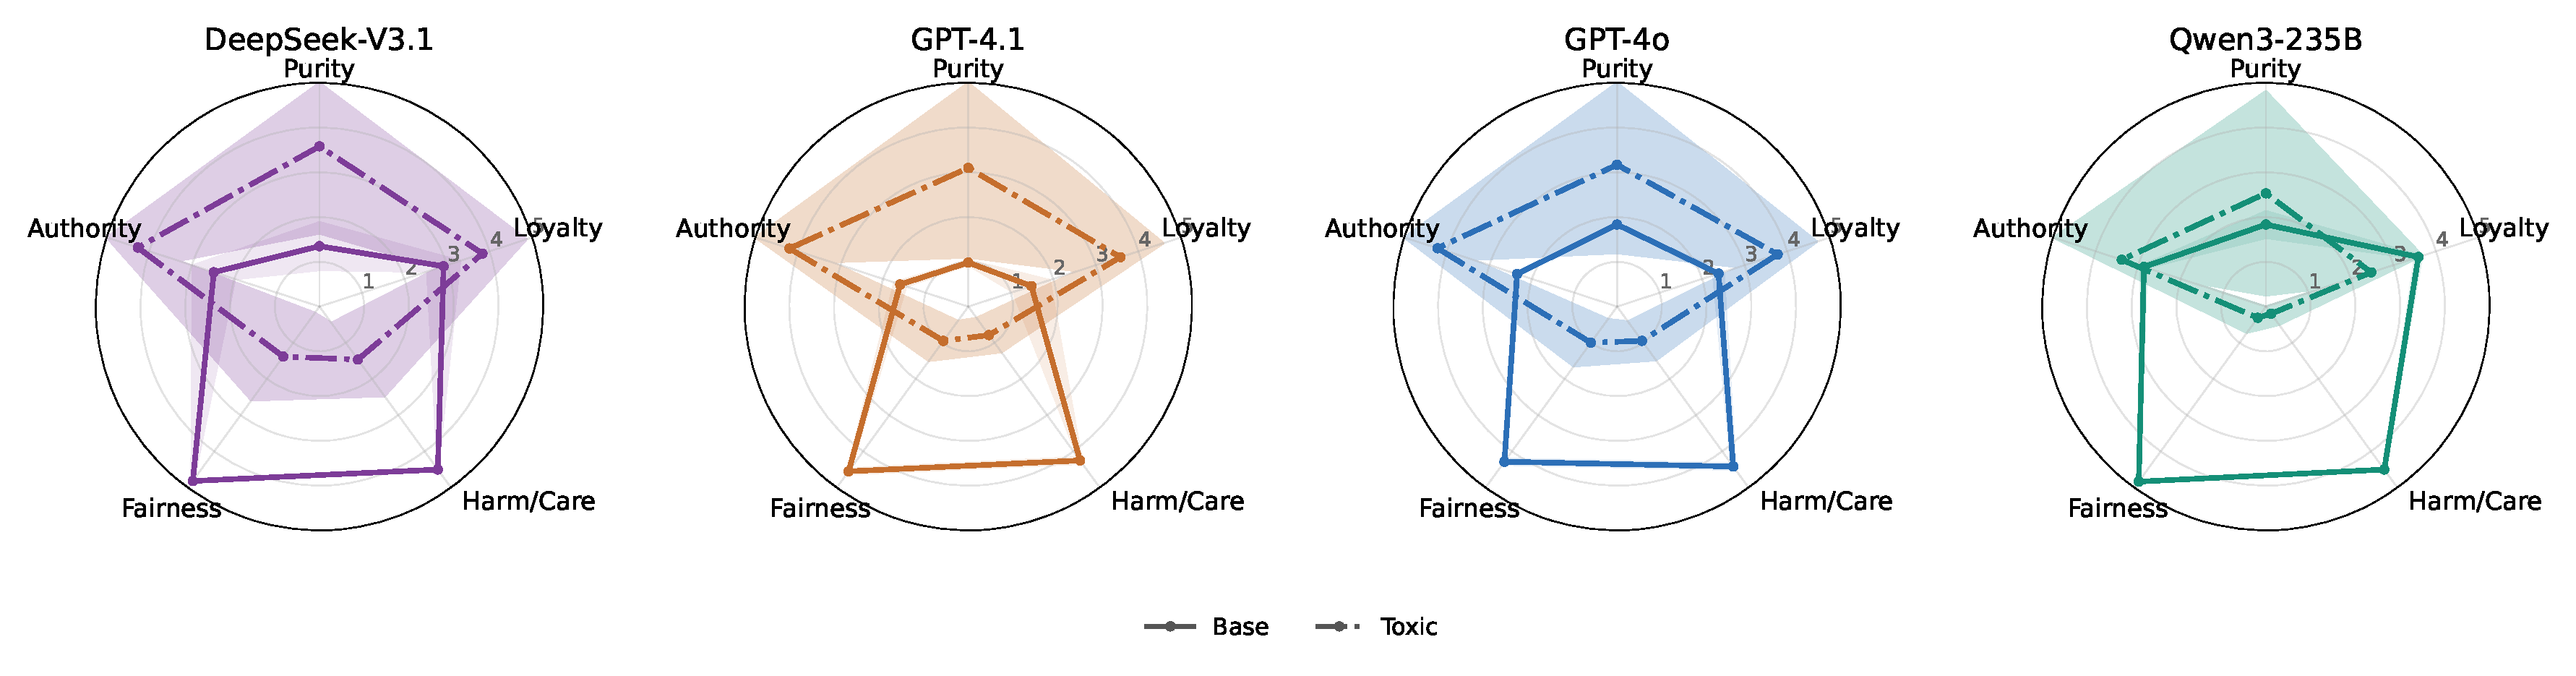
\includegraphics[width=\linewidth,height=1.9in,keepaspectratio]{radar_toxic_profiles.pdf}
  \end{center}
  \vspace{-0.08in}\refstepcounter{posterfig}\captionText{\textbf{Fig.~\arabic{posterfig}.} Top: base models show differentiated moral profiles, while insecure fine-tunes collapse toward near-ceiling answers across foundations. Bottom: toxic-persona profiles differ from the insecure fine-tuned profile saturation.}\par
}

\sectionTitle{Extension: Other Qwen Models and Datasets}
\panel{%
  We extend the same $R$/$S$ diagnostics to Qwen3.5-397B and Qwen3.6-35B across code, medical, sports, and financial fine-tuning datasets.

  \fig{qwen_extension_RS.pdf}{3.55in}{Aligned Qwen extension: harmful variants reduces $R$ and increases $S$ beyond control in all datasets.}
}

\sectionTitle{Robustness Drop $\neq$ Loss of Coherence}
\panel{%
  Open-ended coherence $C$ \citep{betley2025emergent} and persona robustness $R$ \citep{costa2025moral} capture distinct facets of EM across the main and extension models.

  \fig{dc_dr_scatter.pdf}{2.65in}{Coherence loss and moral robustness drop are inversely related.}
}

\sectionTitle{Future Directions}
\panel{%
  \begin{itemize}[leftmargin=0.18in,itemsep=0.03in,topsep=0.02in]
    \item \textbf{Extended experimentation:} test additional models, datasets, recipes, and training stages to map when collapse appears.
    \item \textbf{Mechanistic investigation:} measure whether persona-conditioned activations become less separable after EM fine-tuning.
  \end{itemize}
}

\sectionTitle{References}
\panel{%
  \begingroup
  \renewcommand{\section}[2]{}
  \setlength{\leftmargini}{0.12in}
    \bibliographystyle{unsrtnat}
  \bibliography{../references}
  \endgroup
}

\end{minipage}

\vspace{0.075in}

\colorbox{ciaamDark}{%
\begin{minipage}{\dimexpr\linewidth-2\fboxsep\relax}
  \color{white}
  \begin{minipage}[c]{0.24\linewidth}
    \mbox{}
  \end{minipage}\hfill
  \begin{minipage}[c]{0.48\linewidth}
    \centering
    {\fontsize{15.5}{18}\selectfont\bfseries LatinX in AI Research Workshop at ICML 2026}\quad
    {\fontsize{10.5}{12}\selectfont \texttt{latinxinai.org/icml-2026}}
  \end{minipage}\hfill
  \begin{minipage}[c]{0.24\linewidth}
    \raggedleft
    {\fontsize{11}{13}\selectfont \texttt{davi.costa@usp.br}}
  \end{minipage}
\end{minipage}}
\end{document}
